\section{Acceso remoto.}

En este trabajo se entender� como Acceso Remoto a todo sistema o recurso ubicado f�sicamente en una estancia que realice una acci�n sobre otro en distinto lugar de forma inal�mbrica v�a una red local o externa a trav�s de cualquier medio de comunicaci�n como WiFi, Bluetooth, entre otros.



\subsection{Acceso remoto por RF.}

Cuando se habla de RF, se refiere al espectro de radiofrecuencia contemplado entre los 3Hz hasta 300GHz dentro del espectro electromagn�tico.\\

Al realizar este tipo de dise�o, es necesaria la implementaci�n de circuitos osciladores que logren emitir o recibir la onda de radio que contiene la informaci�n de inter�s. No obstante, con la ayuda de transceptores de radiofrecuencia integrados como el nRF24L01 (Figura \ref{fig:modulorf}) o KYL-500S (Figura \ref{fig:kyl}), se puede realizar el mismo proceso optimizado para el trabajo con microcontroladores.\\


\begin{figure}[H]
	\centering
	\subfigure[KYL-500S. Fuente: Shenzen KYL Communication Equipment Co., Ltd.]{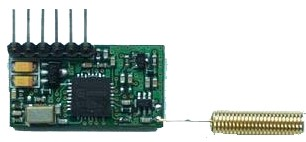
\includegraphics[scale=0.4]{img/kyl}\label{fig:kyl}}
	\subfigure[nRF24L01. Fuente: Nordic Semiconductor.]{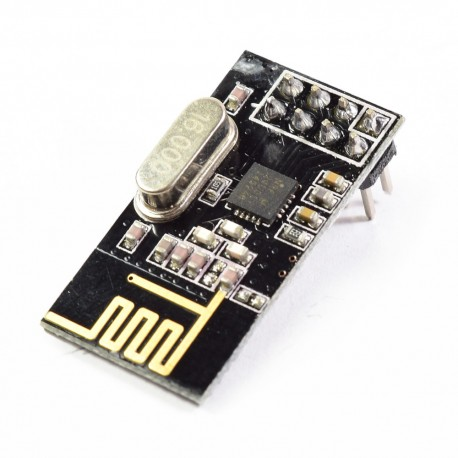
\includegraphics[scale=0.3]{img/modulorf}\label{fig:modulorf}}
	\caption{Algunos transceptores de radiofrecuencia.}
	
\end{figure}

El dise�o de un Acceso remoto por RF debe llevar dos etapas: Transmisi�n y recepci�n. La etapa de recepci�n debe estar conectada al brazo robot, con el inter�s de realizar las m�nimas modificaciones posibles.\\

En cuanto a la etapa transmisora, debe


\subsection{Acceso remoto por Bluetooth.}

\subsection{Acceso remoto por Wi-Fi.}

\subsection{LEGO MindStorm NXT.}

\subsection{QNX Photon}

\subsection{Aplicaci�n de IoT.}
